\chapter{Extended Examples}
\label{examples}
Some extended examples are provided to give a sense of how the \Meta\ environment can be used to enter and evaluate simple expressions, add new constructs to the core language via syntax extension, and build a sub-language for addressing a specific problem.

\section{Entering Expressions}
Here's how the \Meta\ editor can be used to enter some simple expressions.

Suppose you want to evaluate the expression $(1+2) \times 3$. Begin with an empty core-language program, which is a single \keyword{program} node, with no children. The core grammar requires at least one \keyword{doc} or \keyword{expr} node in the program, so the editor supplies an empty node to start you off:
\begin{center}

\includegraphics{src/image/expr1.pdf}
\end{center}
%$$?$$

Select the node and type the character `\clojure{1}'. The editor infers you want to replace the missing node with a new \keyword{int} node in the core language, and does so, leaving the new node selected:
\begin{center}

\includegraphics{src/image/expr2.pdf}
\end{center}
%$$[1]$$

Now we want to add 2 to that, so first type `\clojure{+}'. The editor assumes you want to replace the selected node with a new \keyword{plus} node, and it adds the selected node as the first child of the new node (this is the \emp{insert parent} action with the type \keyword{plus} for the new node). Now the missing right argument is selected:
\begin{center}
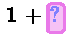
\includegraphics{src/image/expr3.pdf}
\end{center}
%$$1+[?]$$

Simply typing `\clojure{2}' completes the first sub-expression:
\begin{center}
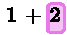
\includegraphics{src/image/expr4.pdf}
\end{center}
%$$1+[2]$$

Now we want to multiply this expression by 3, but you can't simply add the \keyword{times} node yet, because that would make a new node with only 2 as the left argument. Instead, use the ``select parent node'' action (from now on, $\uparrow$) to move the selection to the \keyword{plus} node (or just click on the $+$ sign):
\begin{center}
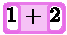
\includegraphics{src/image/expr5.pdf}
\end{center}
%$$[1+2]$$

Now type `\clojure{*}' to create a new node. The previous selection becomes the left child, and \Meta\ inserts parentheses to indicate that the actual grouping of sub-expressions is contrary to what would be suggested by the normal spacing of the operators alone:
\begin{center}
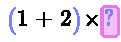
\includegraphics{src/image/expr6.pdf}
\end{center}
%$$\lsyn 1+2 \rsyn \times [?]$$

Finally, type `\clojure{3}' to complete the expression:
\begin{center}
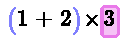
\includegraphics{src/image/expr7.pdf}
\end{center}
%$$\lsyn 1+2 \rsyn \times [3]$$

For this kind of simple expression, the \Meta\ editor's efficiency is quite similar to that of entering text. In fact the sequence of characters is not much different: `\clojure{1+2}$\uparrow$\clojure{*3}' as opposed to, say, `\clojure{(1+2)*3}'. Assuming you use only the keyboard, the actual number of keystrokes is fewer by one with \Meta.

Alternatively, you could have entered the same expression in ``top-down'' fashion using the sequence `\clojure{*+1}$\rightarrow${2}$\uparrow\rightarrow$\clojure{3}'. Interestingly, this seems to mimic the process of typing a prefix expression, with `$\rightarrow$' taking the place of spaces between sibling nodes, and `$\uparrow$' acting as a '\clojure{)}' to close one node and return to the parent. I suspect in practice this is more intuitive than it sounds when described in that way, but only experience will tell (just ask anyone who has learned to use an RPN calculator). The editor attempts to support both styles equally well.

Furthermore, \Meta's rendering of the expression includes appropriate spacing, which you might feel the need to add if you were entering text, maybe like this: `\clojure{(1+2) * 3}' or `\clojure{(1 + 2)*3}', depending on your preference. This kind of manual type-setting is extra work for the programmer (imagine how many hours each year world-wide are spent entering and adjusting white-space!), and it's not very effective anyway. None of the three alternatives is particularly readable.

\vspace{12pt}

The host language provides syntax for more specialized purposes also, and these nodes aren't quite so easily accessed. For example, to generate a list of the first 10 perfect squares, you can use a sequence comprehension. Again, starting with a blank program:
\begin{center}

\includegraphics{src/image/for1.pdf}
\end{center}
%$$[?]$$

Use the \emp{insert node} action to create new node, entering the type \keyword{for}. The new node includes a variable binding. The editor supplies the default name, $x$ (which we won't change):
\begin{center}

\includegraphics{src/image/for2.pdf}
\end{center}
%$$\keyword{for} [x] \leftarrow ? | ?$$

%So just move the selection to the next sibling ($\rightarrow$), and :
For the expression, first enter a variable reference by typing `\clojure{x}'. This inserts a reference to a nearby variable, which happens to be $x$. Alternatively, hold down the \emp{insert reference} modifier keys and click on $x$.
\begin{center}

\includegraphics{src/image/for3.pdf}
\end{center}
%$$\keyword{for} \  x \leftarrow [?] \: .. \: ? \ | \ ?$$

Use the \emp{insert parent} action, entering \keyword{square} for the type:
\begin{center}

\includegraphics{src/image/for4.pdf}
\end{center}
%$$\keyword{for} \  x \leftarrow 1 \: .. \: [10] \ | \ ?$$

Now move the selection to the next sibling twice ($\rightarrow$, $\rightarrow$, or just click on the last `?'). 
\begin{center}
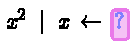
\includegraphics{src/image/for5.pdf}
\end{center}
%$$\keyword{for} \  x \leftarrow 1 \: .. \: 10 \ | \ [x]$$

Insert another node, this time a \keyword{range}.
\begin{center}

\includegraphics{src/image/for6.pdf}
\end{center}

Enter 1 and 10 for the range's min and max:
\begin{center}

\includegraphics{src/image/for7.pdf}
\end{center}

And that's it. Switching to \Meta's evaluation view:
\begin{center}
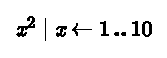
\includegraphics{src/image/for.pdf}
\end{center}

In this case, there is some extra effort to enter the \keyword{for}, \keyword{square}, and \keyword{range} nodes. That's the price of being able to add arbitrary nodes to your language. Furthermore, the editor UI could and should be extended to make this penalty as small as possible, for example, since the keystroke `\clojure{f}' has no particular behavior, it could offer a choice of all known node types beginning with `f'.

These examples hopefully give a sense of how an editor can offer both generality and reasonable usability, but the current \Meta\ editor is certainly only a starting point. Different UI interactions would be appropriate for different kinds of devices (say, emphasizing gestures over keyboard input for a device with a touch-sensitive screen), or for different users (say, something more like a mouse-driven structure editor for end-user programming applications).


%
% Definition of 'for':
%
\section{Defining the Core Language}
\label{for}
The core language is built via syntax extension on top of the kernel language. Several core language nodes provide support for using the primitive cons-list values of the Clojure platform, which are one of the basic tools for organizing data in any Lisp.
These extensions employ a handful of Clojure primitives to expose the native list values of the platform, and the rest of the syntax is built around them.

\begin{figure}[th]
	\centering
	
	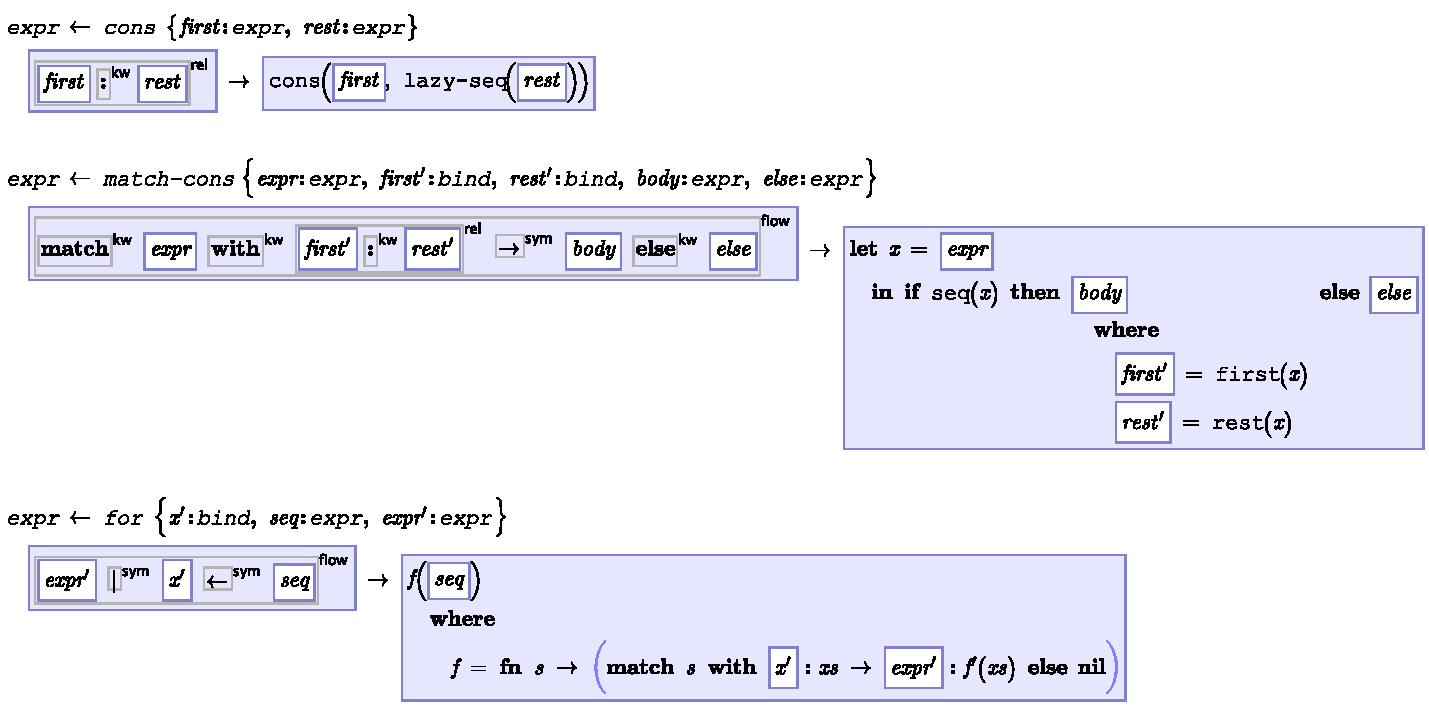
\includegraphics[scale=0.6]{src/image/cons.pdf}
	
	\caption{Declaration of the \keyword{cons}, \keyword{match-cons}, and \keyword{for} node of the core language.}
	\label{fig-for-grammar}
\end{figure}

Figure \ref{fig-for-grammar} shows the declaration of the two primitive constructs for working with with lists, and a node constructed from them. First is the constructor for lists: \keyword{cons}. This node, displayed as a colon operator (as in Haskell), evaluates its \keyword{first} child and uses Clojure's \clojure{cons} function to construct a cons-cell with the resulting value as its head. \clojure{lazy-seq} is applied to the \keyword{rest} child, so that it is not evaluated until the value is needed. This introduces laziness into the core language (recall that the kernel language's semantics is entirely strict), allowing infinite lists to be constructed. Note: the application of \clojure{lazy-seq} is translated by the meta-compiler to an application of the corresponding macro (with no special effort); if \clojure{lazy-seq} was treated as an ordinary (strict) function application, some additional nodes would be required to wrap \keyword{rest} in a lambda abstraction, say, to defer its evaluation.

A \keyword{match-cons} node de-constructs a list. Its children consist of an expression (\keyword{expr}) to be evaluated bindings for the head (\keyword{first}) and the remainder (\keyword{rest}) of the list, an expression (\keyword{body}) to be evaluated if the match succeeds, and an alternative expression (\keyword{else}) to be evaluated if the list is empty. The \emp{expand} reduction implements this by first binding the value of \keyword{expr} to $x$ (a variable local to the reduction), then applying Clojure's \clojure{seq} function, which tests whether the value represents a non-empty list. If so, the two bindings are bound to the parts of the cell using the corresponding Clojure primitive, and the \keyword{body} expression is evaluated.

These two nodes are all that is required to construct a variety of syntax for lists, none of which will need to use the lower-level primitives. As an example, the \keyword{for} (list comprehension) node, used in the previous section, is also defined in Figure \ref{fig-for-grammar}. The \emp{expand} reduction for this node evaluates the \keyword{seq} child, and then applies a recursive function to it. This function attempts to match its argument as a non-empty list (using \keyword{match-cons}). If so, the \keyword{x} child is bound to the first value, and \keyword{expr} is evaluated and then the function is applied to the rest of the list. Note that one of the bindings (\keyword{x}) was supplied by the programmer, and the other ($xs$) is local to the reduction. Both \keyword{x} and $xs$ are in scope when \keyword{expr} is evaluated, thus in the new syntax, the binding introduced by \keyword{x} is in scope in \keyword{expr}, but not in \keyword{seq}.

The rest of the core language's syntax for working with lists is defined in a similar manner, using the \keyword{cons} and \keyword{match-cons} nodes, often in combination with a recursive function to traverse the list. Some examples of the resulting syntax are shown in Figure~\ref{fig-core}. Languages such as Haskell and Python provide such features as integral parts of their fixed grammar and compiler, but in \Meta\ equal or greater expressivity is achieved with a very small implementation effort and with complete modularity---any or all of these nodes can be removed or redefined by simply editing the grammar, without any impact on the rest of the language.


%
% Runtime (enumerating the rationals):
%
\section{Introducing a New Runtime Value}
The preceding section showed how the facilities of the platform can be exposed and wrapped in a novel syntax. This syntax helps the programmer to understand the program, but as soon as the program is reduced to the kernel language for evaluation, the syntax is gone and only the primitive values remain. A more ambitious goal for syntax extension is to augment the language with a new kind of runtime value. This allows programs to operate on a new kind of data, and allows the programmer to see results of computation in the natural form. The next example shows how a new kind of value can be introduced, and how it supports writing a program in a much more natural and comprehensible way.

In a delightful Functional Pearl \cite{gibbons}, Gibbons et al.\ present a series of Haskell programs which generate the infinite series of all positive rational numbers. They begin with the idea of traversing the infinite matrix $a_{ij} = i/j$ which contains every positive ratio, but also contains many equivalent, unreduced ratios (e.g. $\nicefrac{1}{2}$, $\nicefrac{2}{4}$, $\dots$).
%$$
%%\left(
%\begin{array}{cccccc}
%\nicefrac{1}{1} & \nicefrac{2}{1} & \nicefrac{3}{1} & \cdots & \nicefrac{m}{1} & \cdots
%\\
%\nicefrac{1}{2} & \nicefrac{2}{2} & \nicefrac{3}{1} & \cdots & \nicefrac{m}{1} & \cdots
%\\
%\vdots
%\\
%\nicefrac{1}{n} & \nicefrac{2}{n} & \nicefrac{3}{n} & \cdots & \nicefrac{m}{n} & \cdots
%\\
%\vdots
%\end{array}
%%\right)
%$$
%Because every integer appears in the denominator in one column and in the numerator in one row, it's apparent that the matrix contains every positive rational. Concatenating the diagonals
%($\nicefrac{1}{1}$), 
%($\nicefrac{1}{2}$, $\nicefrac{2}{1}$), 
%($\nicefrac{1}{3}$, $\nicefrac{2}{2}$, $\nicefrac{3}{1}$), 
%$\cdots$
%gives an infinite series containing all the rationals, and is easily done in constant space. However, this method has two drawbacks in that the rationals are not in reduced form and each equivalent rational is produced many times (for instance, notice that the diagonal $\nicefrac{1}{1}$, $\nicefrac{2}{2}$, $\nicefrac{3}{3}$, $\cdots$ contains only ratios equal to 1).

The authors show that a series containing all positive rationals in reduced form, without duplicates, is obtained by iterating the function 
$x' = 1/{(\lfloor x \rfloor + 1 - \{x\})}$, beginning with $x=1$.\footnote{In the authors' notation, $\lfloor x \rfloor$ is the floor, or whole-number part of $x$, and $\{x\}$ is the fractional part: $\{x\} = x - \lfloor x \rfloor$, $x > 0$.}This is a surprisingly simple expression, but it is somewhat computationally undesirable in that calculating $\lfloor x \rfloor$ and $\{x\}$ involves division.

%The series begins:
%\begin{eqnarray*}
%&&1
%\\
%(\lfloor 1 \rfloor + 1 - \{1\})^{-1} 
%= (1 + 1 - 0)^{-1} 
%&=& \nicefrac{1}{2}
%\\
%(\lfloor \nicefrac{1}{2} \rfloor + 1 - \{\nicefrac{1}{2}\})^{-1} 
%= (0 + 1 - \nicefrac{1}{2})^{-1} 
%&=& \nicefrac{2}{1}
%\\ 
%(\lfloor 2 \rfloor + 1 - \{2\})^{-1} 
%= (2 + 1 - 0)^{-1} 
%&=& \nicefrac{1}{3}
%\\ 
%(\lfloor \nicefrac{1}{3} \rfloor + 1 - \{\nicefrac{1}{3}\})^{-1} 
%= (0 + 1 - \nicefrac{1}{3})^{-1} 
%&=& \nicefrac{3}{2}
%\\ 
%(\lfloor \nicefrac{3}{2} \rfloor + 1 - \{\nicefrac{3}{2}\})^{-1} 
%= (1 + 1 - \nicefrac{1}{2})^{-1} 
%&=& \nicefrac{2}{3}
%\\ 
%(\lfloor \nicefrac{2}{3} \rfloor + 1 - \{\nicefrac{2}{3}\})^{-1} 
%= (0 + 1 - \nicefrac{2}{3})^{-1} 
%&=& \nicefrac{3}{1}
%\end{eqnarray*}
Interestingly, this formula can be implemented using only ``a constant number of arbitrary-precision integer additions and subtractions, but no divisions or multiplications'' by choosing a different representation for ratios. It happens that the four necessary operations---reciprocal, floor, negate, and fractional part---can all be efficiently performed on ratios represented as \emp{regular continued fractions}. A continued fraction has the form\footnote{Incidentally, this expression is a frequently-cited exception to \TeX's rules for formatting fractions---all the nested expressions are best typeset at the same size, to emphasize the recursive structure. \Meta\ does not provide a way to override that behavior, so continued fractions do not look quite this nice in \Meta!}
$$a_0 + \frac{1}{
    \displaystyle a_1 + \frac{\displaystyle 1}{
        \displaystyle \cdots + \frac{\displaystyle 1}{
            \displaystyle a_n}}}$$
A regular continued fraction is one in which all the coefficients except $a_0$ are positive, and $a_n > 1$ (except for the special case 1). Every rational has a unique representation as a regular continued fraction.

Having arrived at this elegant result, the authors proceed to reduce their formulas to the notation of Haskell for implementation, using lists of integer coefficients to represent continued fractions. In the process, the origins of the code are completely obscured by the loss of the original notation. For example, one of four cases for negation of a regular continued fraction looks like this:\footnote{Actually, what's shown in the paper has been pretty-printed for publication \cite{lhs2tex}. In the actual source code, it must have looked something like this: \clojure{negatecf [n\_0, 2] = [-n\_0-1, 2]}.}
%$$\mathit{negatecf} (n_0 : 1 : n_2 : ns) = (-n_0 - 1) : (n_2 + 1) : ns$$
%$$-\left(n_0 + \frac{1}{\displaystyle 1 + \frac{1}{n_2 + \cdots}}\right) = (-n_0 - 1) + \frac{1}{(n_2 + 1) + \cdots}$$
$$\mathit{negatecf} [n_0, 2] = [-n_0-1, 2]$$
It's up to the reader (of the paper or of the code) to decode the representation of fractions being used here and work out how this corresponds to the algebra that motivated it. However, in the proper notation, the same definition reads as simple algebraic equation which is easily understood and checked:
$$-\left(n_0 + \frac{1}{2}\right) = (-n_0 - 1) + \frac{1}{2}$$

\vspace{12pt}

In \Meta, one can extend the language with a new kind of value for these fractions. I did this by defining a \keyword{continuedFraction} node which defines a recursive data type. It is displayed in the obvious way, except that when the continuation is the ``null'' value, it is displayed in a slightly simplified form. The \emp{expand} reduction is new---it reduces to an expression which evaluates the component expressions and then constructs a node. Therefore the node itself becomes a runtime value. Several \keyword{match} nodes provide pattern matching on the runtime shape of the argument, and are used to identify the cases in each operation. Figure~\ref{fig-cf} shows the declarations of the five operations, and some simple examples of their use are shown in Figure~\ref{fig-cfex}.
\begin{figure}[th]
  \centering
  
%  \todo{split into columns?}
  
  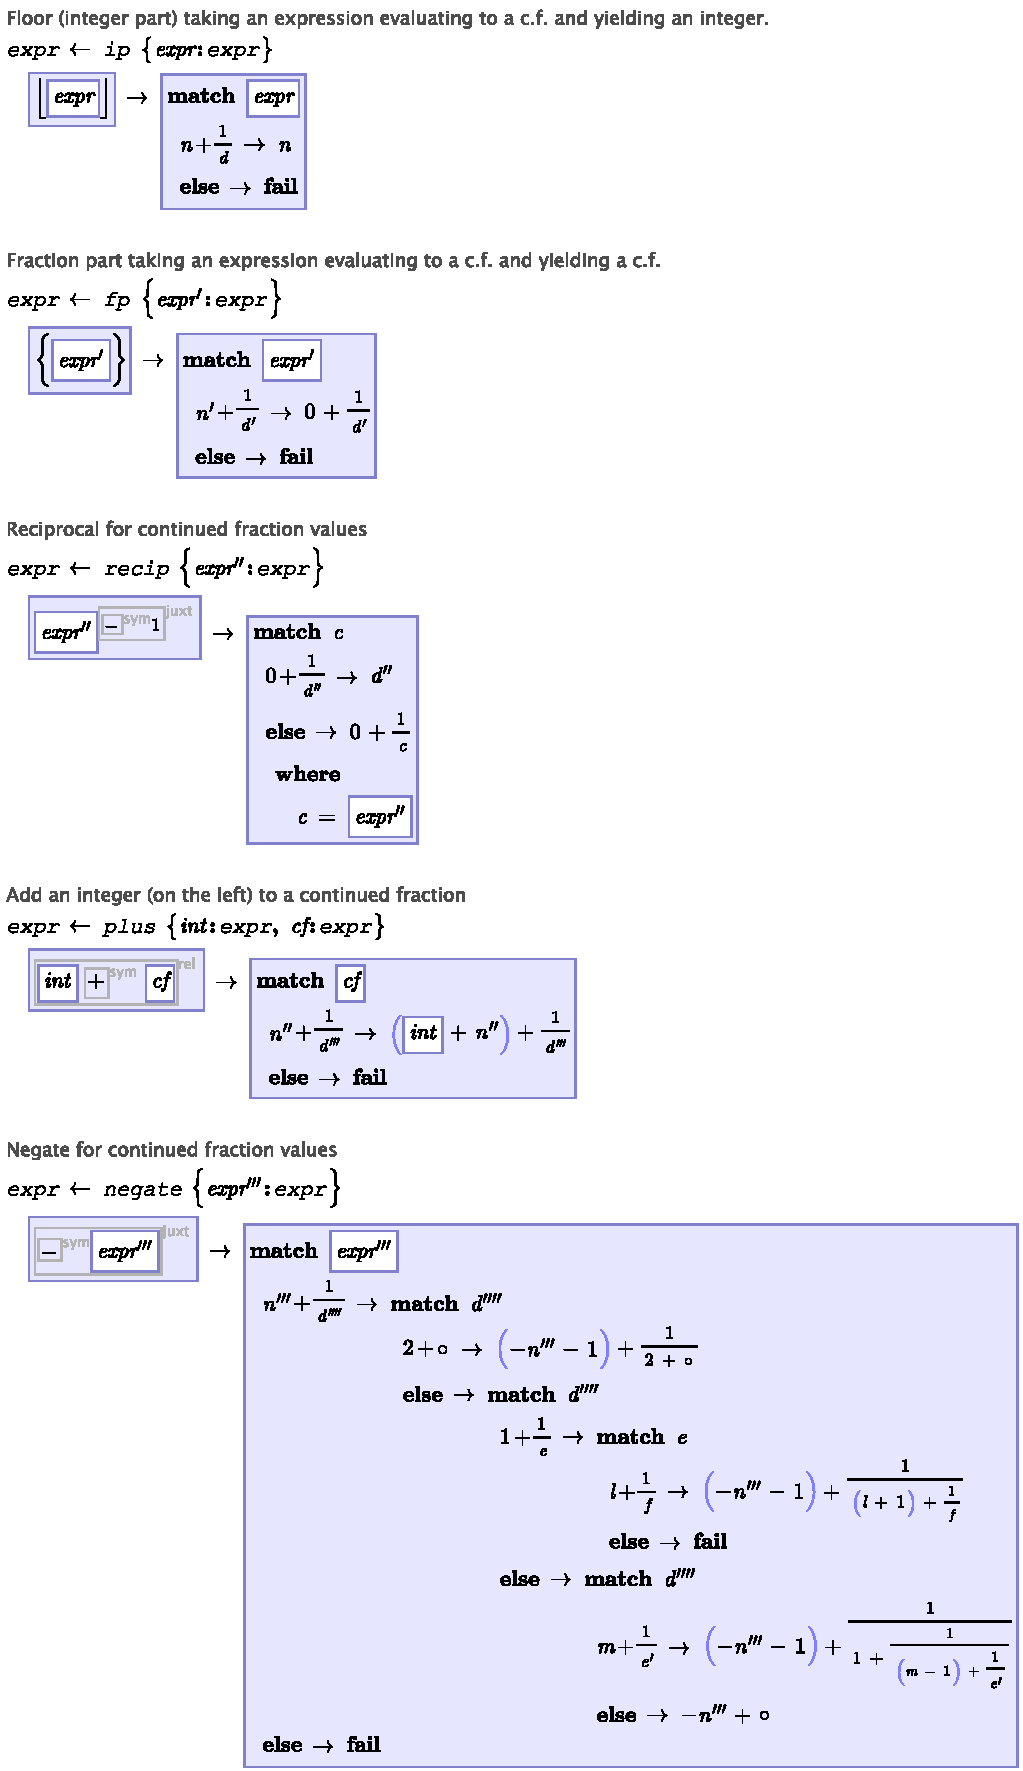
\includegraphics[scale=0.5]{src/image/continued-ops.pdf}
  
  \caption{Grammar for operations on continued fractions as runtime values.}
  \label{fig-cf}
\end{figure}

Note that these declarations are somewhat straining the current capabilities of \Meta. Ideally the construction of a runtime node would be as simple as adding a second level of quotation to the \keyword{expand} reduction, but the current prototype does not handle that properly, so a bit of extra ceremony is required. Likewise, it would be much more convenient to have a general pattern-match construct supporting multiple patterns, each a node with bindings substituted for zero or more of the child nodes, but that is beyond the capabilities of \Meta\ at the moment. Nevertheless, with the hard work of defining syntax and semantics out of the way, the actual algorithm can be expressed quite naturally.

\begin{figure}[th]
  \begin{center}
  
  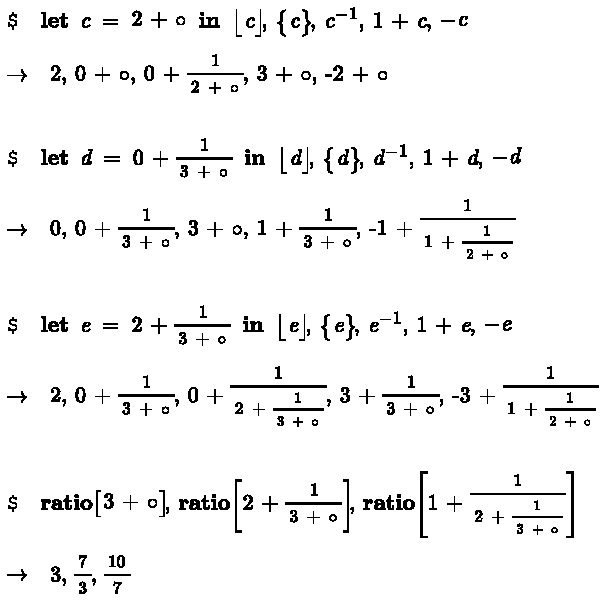
\includegraphics[scale=0.8]{src/image/continued.pdf}
    
  \end{center}
  \caption{Operations on continued fractions.}
  \label{fig-cfex}
\end{figure}

The expression which produces the next fraction in the series, expressed as a function:
\begin{center}
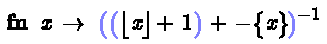
\includegraphics[scale=1]{src/image/rationals-next.pdf}
\end{center}
Note that the exact form of the expression does not match what was shown earlier. Some algebraic manipulation is necessary to put it into a form that uses only the operations that have been defined. The resulting expression contains a node (an operator) for each operation to be performed. For instance, the original expression hid a negation and an addition operation behind a single $-$ symbol, but my version shows both operations.

Other than that, my choice of notation resembles the original closely, but the use of identical $+$ symbols for two distinct addition operations (first addition of integers, and then addition of an integer to a continued fraction) may be confusing. It might be preferable to use a different symbol for the new kind of addition. Because that symbol is specified in one place---the presentation reduction for that node---it's trivial to make the switch. On the other hand, this may be a case where some ambiguity in the visual representation can actually enhance readability. If that freedom leads to an incorrect program, it's easy to click on either node and the editor will indicate which $+$ is of which type.

Now generating the infinite series in continued fraction form is as simple as applying the \emp{iterate} operator (${}^*$) to the $\mathit{next}$ function, using 1 as the initial value:
\begin{center}
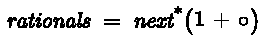
\includegraphics[scale=1]{src/image/rationals-iter.pdf}
\end{center}
The complete expression and the first 15 fractions (converted to simple ratios) appear in Figure~\ref{fig-rationals}. 

% todo: more of a punchline?

\begin{figure}[t]
  \centering
    
  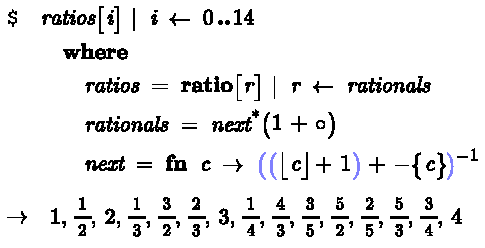
\includegraphics[scale=0.8]{src/image/rationals.pdf}
  
  \caption{Enumerating the rationals, using continued fractions.}
  \label{fig-rationals}
\end{figure}

